% -----
% COMP 3630 Assignment 03
% Jimmy Lin
% -----
% -
%{{{
\documentclass[11pt,a4paper]{article}
\usepackage{geometry}
\usepackage{amsthm}
\usepackage{amsmath}
\usepackage[colorlinks,
            linkcolor=blue,
            anchorcolor=red,
            citecolor=green
            ]{hyperref}
\usepackage{fancyheadings}
\usepackage{graphicx}
\usepackage{tikz}
\usetikzlibrary{automata,positioning}
\geometry{top=18mm,bottom=18mm,left=20mm,right=20mm}
%}}}
% file information
%{{{
\newcommand{\AUTHOR}{Jimmy Lin}
\newcommand{\UID}{u5223173}
\newcommand{\UNIVERSITY}{Australian National University}
\newcommand{\COLLEGE}{College of Engineering and Computer Science}
\newcommand{\COURSE}{COMP3630 Theory of Computation}
\newcommand{\LECTURER}{Jinbo Huang}
\newcommand{\LECTURERt}{Dirk Pattinson}
\newcommand{\TASK}{Assignment 03}
\newcommand{\RELEASEDATE}{May. 7 2013}
\newcommand{\DUEDATE}{May. 20 2013}
\newcommand{\TIMECONSUME}{18h}
%}}}
% new command lst
%{{{
\newcommand{\htab}{\hspace*{0.63cm}}
\newcommand{\dhtab}{\hspace*{1.2cm}}
\newcommand{\ba}{\hspace*{0.2cm} | \hspace*{0.2cm}}
\newcommand{\pg}{\\[0.3cm]}
\newcommand{\lmd}{\underset{lm}{\Longrightarrow}}
\newcommand{\rmd}{\underset{rm}{\Longrightarrow}}
\newcommand{\mlmd}{\overset{*}{\underset{lm}{\Longrightarrow} }}
\newcommand{\mrmd}{\overset{*}{\underset{rm}{\Longrightarrow} }}
\newcommand{\ps}{P_{Stack}}
\newcommand{\pdaid}[2]{(q, #1, #2)}
\newcommand{\idDerive}[1]{\underset{\ps}{\vdash}}
\newcommand{\Y}{Y_{0}}
\newcommand{\LL}{L^{*}}
\newcommand{\lu}{L_{u}}
\newcommand{\clu}{\overline{L_{u}} }
%}}}
%\newcommand{\item}[1]{\hspace*{3cm} #1}
% -
\pagestyle{fancyplain}
\lhead{\COURSE}     
\rhead{\TASK}  
\lfoot{\copyright \AUTHOR (\UID)}
\rfoot{\UNIVERSITY}
% - 
\begin{document}
% ---------------------------
%{{{
\begin{titlepage}
    \begin{center}
        \vspace*{0.8cm}
% add uni photo here.
\includegraphics[width=0.2\textwidth]{/Users/JimmyLin/ANU.png}\\[1cm]
\textsc{\LARGE \UNIVERSITY}\\[1.5cm]

% Title
\rule{\linewidth}{0.5mm} \\[0.4cm]
{ \textsc{\Large \COURSE}\\[0.5cm]
 \huge \bfseries \TASK}\\[0.4cm]
 \footnotesize Edited by \LaTeX \\[0.25cm]
 \normalsize{\COLLEGE}
\rule{\linewidth}{0.5mm} \\[1.5cm]

% other information
\begin{center}
\copyright \emph{\large Author} \\
\Large \textbf{\AUTHOR} \\ \UID \vspace*{0.6cm}

\P \emph{ Lecturer} \\
\Large \textbf{\LECTURER} \vspace*{0.6cm}

\P \emph{ Lecturer} \\
\Large \textbf{\LECTURERt} \vspace*{0.6cm}


$\dagger$ \emph{Release Date}  \\
\Large \textbf{\RELEASEDATE} \vspace*{0.6cm} 

$\ddagger$ \emph{Due Date}  \\
\Large \textbf{\DUEDATE} \vspace*{0.6cm}

$\tau$ \emph{Time Spent} \\
\Large \textbf{\TIMECONSUME} \vspace*{0.6cm} 
\end{center}
% foot
\vfill
{\large \today}
\end{center}
\end{titlepage}

% table of content
\begin{center} \tableofcontents \end{center}
 \newpage
%}}}
% --------------------------
% Exercise 1 
%{{{
\section{Turing Machine Design}
Design a Turing machine that shifts the entire input string to the right by one place, under the following conditions: The input alphabet is $\{0, 1\}$ and the Turing machine has a single tape with a single track. Describe the Turing machine in words, and draw its transition diagram.
\subsection{Describe the Turing machine in words}
\htab Since the functionality of the desired Turing Machine is to shift the entrie input string to the right by one place, it is not applicable to directly read symbol from left cell, sweep it and write to the right-neighboured cell (the right one would be covered).\\
\htab Rather, we should first move the head of tape rightward without changing any symbol until meeting the first blank cell and then execute the copy task leftward recursively. After that, in order to copy content of each cell to the neighbour cell on its right, obviously, we ought to sweep the objective cell, and move right. Then write down the recorded symbol and move back to the objective cell. Finally move left to the next objective cell and repeat the copy task described above if the symbol in the tape is not blank. \\
\htab Note that since only one memory device is allowed, we have to use state to record what symbol we have just read, and it is also practical to apply this approach for an alphabet with only two characters.
\subsection{Draw the transition diagram}
\htab The transition diagram is shown in the following figure, 
\begin{center}
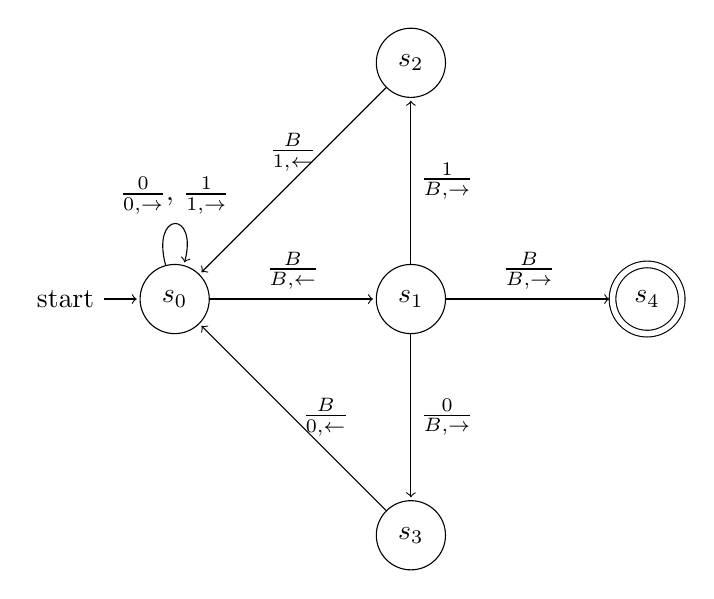
\begin{tikzpicture}[shorten >=1pt,accepting/.style={double distance=2pt},node distance=3cm,on grid,auto,bend angle=45] 
   \node[state,initial] (s0)   {$s_0$}; 
   \node[state] (s1) [right=of s0] {$s_{1}$}; 
   \node[state] (s2) [above=of s1] {$s_{2}$}; 
   \node[state] (s3) [below=of s1] {$s_{3}$}; 
   \node[state,accepting](s4) [right=of s1] {$s_4$};
   \path[->] (s0) edge [loop above] node {$\frac{0}{0,\rightarrow}$, $\frac{1}{1,\rightarrow}$} (s0);
   \path[->] (s0) edge  node  {$\frac{B}{B,\leftarrow}$} (s1);
   \path[->] (s1) edge [above]  node  {$\frac{B}{B,\rightarrow}$} (s4);
   \path[->] (s1) edge [right] node  {$\frac{1}{B,\rightarrow}$} (s2);
   \path[->] (s1) edge [right] node  {$\frac{0}{B,\rightarrow}$} (s3);
   \path[->] (s2) edge [above] node  {$\frac{B}{1,\leftarrow}$} (s0);
   \path[->] (s3) edge [right] node  {$\frac{B}{0,\leftarrow}$} (s0);
\end{tikzpicture}\\[0.5cm]
\footnotesize Fig. TM $M_{0}$ with acceptance by final state
\end{center}
\htab Note that when we first sweep the cell to blank symbol (see $s_{1}$) before copying its content to the adjacent right cell. In this manner, it is unnecessary to specify more transitions because the cell we just copy must be blank (when copy task starts up, TM $M$ must read blank symbol at state $s_{0}$ because we sweep the cell whose content is just copyed. And in $s_{2}$ and $s_{3}$, only blank symbol will be read.). Finally, we terminate the Turing Machine when there is blank symbol to read at state $s_{1}$.
\newpage
%}}}
% Exercise 2 
%{{{
\section{Enumerating a Recursively Enumerable Language}
Given a Turing machine M that accepts a language $L$, informally but clearly show that a Turing machine $M′$
can be constructed to enumerate all members of L in the following sense: \\
    \htab (i) Whenever $M'$ enters a special state p, the string to the left of the tape head is a member of $L$. \\
    \htab (ii) Every member of $L$ appears on the tape at some point in the aforementioned way.  \\
Keep in mind that the Turing machine $M$ may not halt on all inputs.
\subsection{Construct special TM $M'$}
\htab The diagram that summarises the description of construction is shown in the following.
\begin{center}
\includegraphics[width=5in,height=1in]{./TM2.png} \\
\footnotesize Fig.2. Construction for Turing Machine $M'$
\end{center}
\htab Note that the special state $p$ in our proposal is instantiated to be the accepting state of $M'$. 
And Turing Machine $M'$ use the same tape to simulate all three TMs, $M$, $M_{rev}$, $M_{R}$.\\
\htab Specifically, construct the Turing Machine $M'$ as follows: 
\begin{itemize}
    \item{Ignore its own input $x$ and Guess arbitrary $w$}
    \item{Simulate given TM $M$ on guessed string $w$. The functionality of TM $M$ here is to disable the 
            TM $M'$ with the string $w$ that is not accepted by given TM $M$.}
        \begin{itemize}
            \item{if the accepting state of $M$ is reached, which means $w \in L(M)$,
                    TM $M'$ starts to simulate TM $M_{rev}$ using the same tape. (tape symbols and tape 
                head remained unchanged and are used as input of $M_{rev}$)}
            \item{If the accepting state of $M$ is never reached, that is, $w \notin L(M)$. Therefore, it would be impossible to for TM $M'$ to enter its accepting state.}
        \end{itemize}
    \item{Simulate $M_{rev}$ if activated. And the TM $M_{rev}$ is constructed by the reversing all the transitions of $M$, make start state of $M$ as accepting state and replace accepting state of $M$ to be start state. The functionality of TM $M_{rev}$ is to recover the original input $w$ to TM $M$. }
        \begin{itemize}
            \item{For all strings that are input to $M_{rev}$ with specific position of tape head, the accepting state of $M_{rev}$ will be reached, that is, they must be accepted by $M_{rev}$.}
                \end{itemize}
            \item{Simulate $M_{R}$ if activated. The TM $M_{R}$ is designed to move the tape head of TM $M'$ rightward until it meets first blank symbol. This is easy to simulate. In this manner, the recovered string $w$, which is accepted by $M$ can be in the left of tape head.}
        \begin{itemize}
            \item{If TM $M_{R}$ meets first blank symbol, goes into 
                accepting state of $M_{R}$ and trigger the acceptance of TM $M'$.}
        \end{itemize}  \end{itemize} 
\htab Next explain why the Turing Machine $M'$ we just construct satisfies the requirement (i) and (ii).\\
\htab For requirement (i). Since only if guessed string $w \in L(M)$, $w$ will make $M$ into its accepting state, thereby activating $M_{rev}$, and all $w$ that activates $M_{rev}$ would lead $M_{rev}$ to its accepting state, it can be derived that the string $w$ will activate $M_{R}$ only if $w \in L(M)$. Since all strings that activate $M_{R}$ will lead $M_{R}$ to accepting state and thus trigger acceptance of $M'$, combined with the fact that  $M_{R}$ only move the position of the tape head without changing cells' content. Therefore, if TM $M'$ enter its accepting state, the guessed $w$ must be in $L(M)$.\\
\htab For requirement (ii). TM $M'$ will guessed all possible strings in the very beginning. And if the guessed 
string $w \in L(M)$, as described in specfication of $M'$, this string will definitely pass the filtering TM $M$, 
then be recovered by $M_{rev}$ and finally be set in the left of tape head of $M'$ by $M_{R}$. \\
\newpage
%}}}
% Exercise 3 
%{{{
\section{Proving Undecidability}
Consider the following theorem and attempted proof thereof. Identify the flaw in the attempted proof, and give a correct proof. \\
\textbf{Theorem}: The set of all (encodings of) Turing machines that have a \textit{useless} state 
is undecidable, where a useless state is defined as a state that is never visited on any input string. \\
\textbf{Attempted proof (sketch)}: Reduce the universal language to this problem. Given $(M, w)$,
construct a Turing machine Q that replaces its input string with $(M, w)$, simulates the universal
Turing machine, and enters the accepting state $q_{accept}$ if and only if the (simulated) universal
Turing machine accepts $(M, w)$. The reduction works as the Turing machine Q will have a useless
state ($q_{accept}$) if and only if the Turing machine $M$ does not accept the string $w$. 
\subsection{Flaw of attempted proof}
\textbf{Flaw}: The reduction did not relate the problem of whether given TM $M$ accept certain 
string $w$ to our objective problem, which is whether one coded TM will have useless state. Specifically,
if $M$ accept the string $w$, the accepting state of $Q$ will be reached, which means $q_{accept}$ is not
 useless. But under this circumstance, we still have no idea about whether the TM $Q$ has useless state.
 (there may exist some other states of TM $Q$ to be useless or may not.) Therefore, what 
 the reduction in the attempted proof do is to relate the problem of whether TM $M$ accepts string
 $w$ to the problem of whether accepting state of $Q$, $q_{accept}$ is useless state, but not our 
 objective problem, that is, whether the TM $Q$ has a useless state. 
\subsection{Correct Proof}
 \textbf{Correct Proof}: We first will prove that the Turing Machine $M_{c}$ which take 
 a pair of coded TM and one state from that TM as input is undecidable by reducing $\lu$ to 
 $L(M_{c})$. And then we reduce to the problem of given TM and one state of that TM, whether 
 the state is useless state to the problem of whether a TM has one useless state. \\
 \htab Assume that there is a TM $M_{c}$ decide the language $L_{c}=\{(M,q)\ba \text{q is useless state in TM }M\}$.
 By this assumption, we can reduce the $\lu$ to $L_{c}$, and show that if there exist a $M_{c}$ decide
 the $L_{c}$, there must be one TM $M'$ to decide $\lu$. We construct the  
 Turing Machine $M'$ by using $M_{c}$ as follows.
 \begin{center}
 \includegraphics[width=5in,height=1.5in]{./TM3.png} \\
 \footnotesize Fig.3. Construction for $M'$ using $M_{c}$
 \end{center}
 \htab Note that TM $M'$ does not run $M_{test}$ but just produces the code of TM $M_{test}$. \pg
 \htab Description for the constructed $M'$ is as follows
 \begin{itemize} 
     \item{What TM $M'$ do in first step is to generate the coded TM $M_{test}$. The TM $M_{test}$ has
         its own input $x$. But $M_{test}$ ignore its input $x$ and simulate $M$ on string $w$. If 
     $M$ accepts string $w$, then $M_{test}$ accepts $(M,w)$. Note that if $M$ does not accept $w$,
 $M_{test}$ may not halt, but here we do not run $M_{test}$, just generate code of $M_{test}$.}
     \item{Let $q$ be the accepting state of $M_{test}$. }
     \item{Simulate $M_{c}$ on $(M_{test}, q)$. If $M_{c}$ rejects, $M'$ goes to accepting state. 
         If $M_{c}$ accepts, $M'$ halts on non-accepting state. (note that this is valid because
     we have assumed that $M_{c}$ is decidable.)}
 \end{itemize}
 \htab As we can see, $M'$ is a TM taking $(M,w)$ as its input. And $M'$ accepts iff $w \in L(M)$. 
 Conversely, $M'$ rejects iff $w \notin L(M)$. (for those $w \notin L(M)$, TM $M'$ always halts).
 That is to say, $M'$ can decide the $\lu= \{(M,w)\ba w\in M \}$, which contradicts the theorem 
 that universal language $\lu$ is not decidable. Thus, we should negate the original assumption 
 to have the following conclusion. 
 \begin{align}
     L_{c}=\{(M,q)\ba \text{$q$ is useless state in TM $M$ is undecidable} \}. 
 \end{align}
 \htab After acquiring a fairly important conclusion, let's go back to prove the undecidability of 
 $L_{a} = \{ M \ba M \text{ has at least one useless state.}\}$ It is evident that we achieve the
 proof by reducing $L_{c}$ to $L_{a}$. The specific way is as follows. \\
 \htab Given a TM $M$, to know whether this TM has a useless state, we can traverse all the state 
 of TM $M$, and ask $M_{c}$ whether $q_{i}$ in TM $M$ is a useless state. The final result to the 
 question of whether TM $M$ has one useless state is "no", if and only if all the answers from
 $M_{c}$ are "no". Conversely, the result to taht question is "yes" if and only if 
 there is one "yes" from $M_{c}$. Therefore, $L_{c}$ is reducible to $L_{a}$ in polynomial time.
 And since we have proven that $L_{c}$ is undecidable, we can conclude that $L_{a}$ is also undecidable.
\newpage
%}}}
% Exercise 4 
%{{{
\newcommand{\lie}{L_{ie}}
\newcommand{\lnw}{L\big(N(w)\big)}
\section{Proving Non-Recursive Enumerability}
Show that the following is not recursively enumerable: $\{(M_{1}, M_{2}) \ba L(M_{1}) \cap L(M_{2}) = \emptyset \}$, i.e., the set
of pairs of Turing machines the intersection of whose languages is empty. \pg
\htab First of all, we name the objective language to be $\lie$ (subscript means intersection is empty). Formally,
\begin{align}
    \lie = \{(M_{1}, M_{2}) \ba L(M_{1}) \cap L(M_{2}) = \emptyset \}
    \end{align}
\htab it should be illustrated the property of complement of universal language and universal language. That is,  $\clu = \{ (M,w) \ba w \notin L(M) \}$ is not recursively enumerable since $\lu = \{ (M,w) \ba w \in L(M)\}$ is recursively enumerable but not recursive. Thus, there is no Turing Machine accepting language $\clu$ since it is non-RE. \\
\htab Assume that $\lie$ is recursively enumerable. And suppose one Turing Machine $Q$ that accept the objective language $\lie$. \\
\htab Then we start to construct one Turing Machine $M_{new}$ to relate the binary coded string $(M,w)$ to 
the Turing Machine $Q$. \\
\htab Let $M_{new}$ translate input string $w$ to one Turing Machine $N(w)$ that only accept $w$ itself, that is
\begin{align}
    \lnw = \{ w \} \label{4:110}
    \end{align}
\htab Note that the way to construct such a $w$ can be just to compare the character of its input 
 one-by-one with a stored copy of $w$. \\
\htab Next we apply the property of the Turing Machine $Q$, which is assumed in the very beginning. That is,
\begin{align}
    L(M) \cap \lnw = \emptyset
    \end{align}
\htab By what we derived in \eqref{4:110}, we have
\begin{align}
    L(M) \cap \{w\} = \emptyset
    \end{align}
    \htab which is tantamount to the following equation since $w$ is the only element of set $\{w\}$,
\begin{align}
    w \notin L(M)
    \end{align}
\htab that is,
\begin{align}
    L(M_{new}) = \{ (M, w) \ba w \notin L(M) \}
    \end{align}
\htab which means $M_{new}$ accept the language $\clu$, which contradicts our previous statement that
there exists no Turing Machine accepting $\clu$. Therefore, we should negate the assumption and have
\begin{align}
    \text{ $\lie$ is not recursively enumerable}.
   \end{align}
\newpage 
%}}}
% Exercise 5 
%{{{
\newcommand{\x}[1]{x_{#1}}
\newcommand{\n}[1]{\overset{-}{x_{#1}} }
\section{Boolean Encodings of Graph Properties}
Suppose $G$ is an undirected graph of four nodes: 1, 2, 3, and 4. Let $x_{ij}$ , for $1 \leq i < j \leq 4$,
be a Boolean variable that we interpret as saying “there is an edge between nodes i and j.”
The expression $x_{12}x_{23}x_{34}x_{14} + x_{13}x_{23}x_{24}x_{14}+x_{13}x_{34}x_{24}x_{12}$, for example, 
says that the graph G has a Hamilton circuit. In general, a Boolean expression over 
the $x_{ij}$ variables describes a property of the graph in the sense that a truth assignment
to the variables satisfies the expression if and only if it describes a graph having 
that property. Write expressions for the following properties:
\begin{itemize}
    \item{1. G contains a clique of size 3 (i.e., a triangle). }
    \item{2. G contains at least one node with no edges. }
    \item{3. G is connected.}
\end{itemize}
\subsection{G contains a clique of size 3}
\htab Obviously, all graphs that has clique of size three must have one of four possible triangles. \\
\begin{align}
    \x{12}\x{23}\x{13} ,\
    \x{23}\x{34}\x{24} ,\  
    \x{34}\x{14}\x{13} ,\
    \x{14}\x{12}\x{24} 
\end{align}
\htab Therefore, the following boolean expression would be evaluated to be true
if and only if the graph $G$ contains a clique of size 3, that is
\begin{equation}
\begin{aligned}
    &\htab    \x{12}\x{23}\x{13} +
    \x{23}\x{34}\x{24}  + 
    \x{34}\x{14}\x{13} + 
    \x{14}\x{12}\x{24} \end{aligned}
\end{equation}
\subsection{G contains at least one node with no edges}
\htab Before providing solution to this question, we first introduce one notation $\n{ij}$, which
means there is no edge from node $i$ to node $j$. \\
\htab For all graphs that at least one node has no edges must satisfy one of following boolean term. 
Each of boolean term shown in the followings represents one possible node with no edge.
\begin{equation}
\begin{aligned}
    \n{12}\n{13}\n{14} ,\ 
    \n{23}\n{24}\n{12} ,\ 
    \n{34}\n{23}\n{13} ,\ 
    \n{14}\n{24}\n{34} ,\ 
\end{aligned}
\end{equation}
\htab Since any graph that has more than one still needs to satisfy one of boolean terms shown above,
we have the following boolean expression, which is true if and only if graph $G$ contains at least
one node with no edges.
\begin{equation}
\begin{aligned}
    \n{12}\n{13}\n{14} + 
    \n{23}\n{24}\n{12} + 
    \n{34}\n{23}\n{13} + 
    \n{14}\n{24}\n{34}  
\end{aligned}
\end{equation}
\subsection{G is connected}
\htab Easy to see that all graph with more than $3$ edges must be connected and that all graph with less
than $3$ edges must be non-connected. Thus, we only need to discuss the boolean expression
based on those graphs with $3$ edges. \\
\htab Specifically, simplified boolean expression for all connected graphs are presented as follows,
\begin{equation}
\begin{aligned} 
    &\htab 
    % 3 terms: 16
    \x{12}\x{13}\x{24} +
    \x{23}\x{13}\x{24} +
    \x{34}\x{13}\x{24} +
    \x{14}\x{13}\x{24} \\&+
    %
    \x{12}\x{14}\x{13} +
    \x{23}\x{34}\x{13} +
    \x{23}\x{14}\x{13} +
    \x{12}\x{34}\x{13} \\&+
    \x{34}\x{14}\x{24} +
    \x{12}\x{14}\x{24} + 
    \x{23}\x{14}\x{24} +
    \x{12}\x{34}\x{24} \\&+
    %
    \x{23}\x{34}\x{14} +
    \x{12}\x{34}\x{14} +
    \x{12}\x{23}\x{14} +
    \x{12}\x{23}\x{34}
\end{aligned}
\end{equation}
\newpage
%}}}
% Exercise 6
%{{{
\newcommand{\NP}{\mathcal{NP}}
\section{Proving $\NP$-Completeness}
We know that the Node Cover problem is $\NP$-complete.
Show that the following Dominating Set problem is $\NP$-complete: Given a graph $G$ 
and an integer $k$, does there exist a subset $S$ of at most $k$ nodes of G such that 
each node is either in $S$ or adjacent to a node of $S$? 
\subsection{Dominating problem is in $\NP$}
\htab To prove the the Dominating Set Problem is in $\NP$, we can show one non-deterministic Turing Machine to achieve
the task of figuring out whether there is a dominating set with at most $k$ nodes in given graph $G$. \\
\htab The non-deterministic Turing Machine works as follows. Non-deterministically choose ("guess") $k$ nodes from given graph $G$ and form nodes set $S$. The time complexity for this step is $O(klog(n))$. Then check whether all the nodes are in chosen set $S$ or adjacent to nodes set $S$. This step will cost $O(n^{3}k)$ in worst case. Once we find one node that is neither in set $S$, nor adjacent to node set $S$, we reject the given graph and $k$. If the dominating set exists, there should be one execution path by which we successfully "guessed" the dominating set and accept. Since the whole algorithm runs in polynomial time, so dominating problem is in $\NP$.
\subsection{Node Cover Problem reduction}
\htab Now we describe the reduction from the Node Cover Problem to Dominating Set Problem. \\
\htab Given a graph $G$, we can replace each edge in $G$ by one triangle to create graph $G'$. Formally, new graph $G' = (V',E')$, where the set of nodes $V'= V \cup V_{e}$ and the set of edges $E' = E \cup E_{e}$. Specifically, $E_{e} = \{ (v_{e_{i}}, v_{k}), (v_{e_{i}}, v_{l}) | e_{i} = (v_{k}, v_{l}) \in E\}$, and $V_{e} = \{ v_{e_{i}}, e_{i} \in E\}$. \\
\htab Next we first claim and then prove that 
\begin{align}
    \text{graph $G$ has cover set of size $K$ \textbf{if and only if} the graph $G'$ has dominating set of size $k$}
\end{align}
\htab (If part) If $G$ has a node cover $S$ of size $K$, then the same set of nodes form a dominating set in $G'$. This is because for each edge $(u,v)$ in graph $G$, either $u$ or $v$ must be in the dominating cover consisting of those $K$ nodes, otherwise the $K$-node-cover property of graph $G$ does not hold. And the transformation by replacing edge with triangle will not introduce any inadjacency. That is, for each edge, whatever $u$ or $v$ is in the cover set, newly introduced node $x$ is always adjacent to the node that is in cover set. \\
\htab (Only-if part) Suppose that there is a dominating set of size $K$ in graph $G'$. We can specify that dominating set only pick up nodes from the set $V$. If $v_{e_{i}}$ was picked, we can replace it by $v_{k}$ or $v_{l}$ without increasing its size and changing its nature of being a dominating set. In this manner, for each edge $e_{i}$, $v_{e_{i}}$ must have neighbour, either $v_{k}$ or $v_{l}$ in the dominating set. Then, the node $v_{e_{i}}$, edge $(v_{e_{i}}, v_{l})$ and edge $(v_{e_{i}}, v_{k})$ can be removed to derive the original graph $G$ with a node cover of size $K$. The resulted graph has a node cover of size $k$ because we have claimed that, for each triangles, only one edge $(v_{k}, v_{l})$ was reserved and either $v_{k}$ or $v_{l}$ is in the dominating set. Thus, the dominating set in $G'$ is the node cover set in graph $G$. \pg
\htab In summary, since the Dominating Set Problem is in $\NP$ class and the Node Cover Problem, which has been proven to be $\NP$-complete, can be reducible to Dominating Set Problem, it can be concluded that Dominating Set Problem is $\NP$-complete.
%}}}
\end{document}
%{{{ wrong answer

\subsection{G contains a clique of size 3}
\htab Enumerate all possible expressions by extracting $0,1,2$ edges in the external square. \\
\htab For the case of number of the non-existing edges in external square is $0$, we have two boolean terms
\begin{equation}
\begin{aligned}
    \x{12}\x{23}\x{34}\x{14}\x{13} ,\
    \x{12}\x{23}\x{34}\x{14}\x{24} 
\end{aligned}
\end{equation}
\htab For the case of number of the non-existing edges in external square is $1$, we have eight boolean terms
\begin{equation}
\begin{aligned}
     \x{12}\x{23}\x{34}\x{13} ,\
    \x{12}\x{23}\x{34}\x{24} \\
     \x{12}\x{23}\x{14}\x{13}  ,\
    \x{12}\x{23}\x{14}\x{24} \\
    \x{12}\x{34}\x{14}\x{13}  ,\
    \x{12}\x{34}\x{14}\x{24} \\
     \x{23}\x{34}\x{14}\x{13} , \
    \x{23}\x{34}\x{14}\x{24} 
\end{aligned}
\end{equation}
\htab For the case of number of the non-existing edges in external square is $2$, we have four terms
\begin{align}
    \x{12}\x{23}\x{13} ,\
    \x{23}\x{34}\x{24} ,\  
    \x{34}\x{14}\x{13} ,\
    \x{14}\x{12}\x{24} 
\end{align}
\htab In summary, there are in total $2+8+4 = 14$ cliques and we can sum up all those boolean terms to
acquire the boolean expression showing that G contains a clique of size 3, that is
\begin{equation}
\begin{aligned}
    &\htab \x{12}\x{23}\x{34}\x{14}\x{13} +
    \x{12}\x{23}\x{34}\x{14}\x{24} +
    \x{12}\x{23}\x{34}\x{13} \\&+
    \x{12}\x{23}\x{34}\x{24} +
     \x{12}\x{23}\x{14}\x{13}  +
    \x{12}\x{23}\x{14}\x{24} + 
    \x{12}\x{34}\x{14}\x{13}  \\&+
    \x{12}\x{34}\x{14}\x{24} +
     \x{23}\x{34}\x{14}\x{13} + 
    \x{23}\x{34}\x{14}\x{24} +
    \x{12}\x{23}\x{13}  \\&+
    \x{23}\x{34}\x{24} +   
    \x{34}\x{14}\x{13} +
    \x{14}\x{12}\x{24} 
\end{aligned}
\end{equation}
\subsection{G contains at least one node with no edges}
\htab Enumerate all possible expressions over $1,2,3,4$ nodes with no edge. \\
\htab For the case of number of the non-existing edges in external square is $1$, 
we have $4 \times 4 = 16$ boolean terms
\begin{equation}
\begin{aligned}
    \x{12}\x{23}\x{13} ,\
    \x{12}\x{13} ,\
    \x{12}\x{23} ,\
    \x{23}\x{13} \\
    \x{23}\x{34}\x{24} ,\
    \x{23}\x{24} ,\
    \x{23}\x{34} ,\
    \x{34}\x{24} \\
    \x{34}\x{14}\x{13} ,\
    \x{14}\x{13} ,\
    \x{34}\x{13} ,\
    \x{34}\x{14} \\
    \x{14}\x{12}\x{24} ,\
    \x{14}\x{12} ,\
    \x{12}\x{24} ,\
    \x{14}\x{24} 
\end{aligned}
\end{equation}
\htab For the case of number of nodes with no edge is $2$, we have $4 + 2 = 6$ boolean terms
\begin{equation}
\begin{aligned}
    \x{12} ,\
    \x{23} ,\
    &\x{34} ,\
    \x{14} \\
    \x{13} ,\
    &\x{24}
\end{aligned}
\end{equation}
\htab For the case of number of nodes with no edge is $3$, we have no boolean terms. \\
\htab For the case of all node have no edge, we have only one boolean term
\begin{align}
    \epsilon
\end{align}
\htab where we utilise $\epsilon$ to denote the case where no connected edge exists in graph G. \\
\htab In summary, there are in total $16 + 6 + 0 + 1 = 23$ boolean terms satisfying given requirement
and we can sum up all those boolean terms to acquire the boolean expression showing that 
G contains at least one node with no edges, that is
\begin{equation} \label{5:second}
    \begin{aligned}
    & \ \ \ \x{12}\x{23}\x{13} +
    \x{12}\x{13} +
    \x{12}\x{23} +
    \x{23}\x{13} \\ & + 
    \x{23}\x{34}\x{24} +
    \x{23}\x{24} +
    \x{23}\x{34} +
    \x{34}\x{24} \\ & +
    \x{34}\x{14}\x{13} +
    \x{14}\x{13} +
    \x{34}\x{13} +
    \x{34}\x{14} \\& +
    \x{14}\x{12}\x{24} +
    \x{14}\x{12} +
    \x{12}\x{24} +
    \x{14}\x{24} \\& +
        \x{12} +
    \x{23} +
    \x{34} +
    \x{14} +
    \x{13} +
    \x{24} +
    \epsilon
\end{aligned} 
    \end{equation}
\subsection{G is connected}
\htab To derive the boolean expression that presents the connectivity property of G,
theoretically, we are expected to get $2^{6}-23-3 =64-23-3= 38$ boolean terms 
since desired boolean expressions should contain all boolean terms that does not appear 
in the solution of last question \eqref{5:second} except three special cases. \\ 
\htab Those special cases we need to remove from our answer is the terms where all nodes
has at least one edge and are not connnected. Specifically, they are
\begin{align}
    \x{13}\x{24},\ \x{12}\x{34},\ \x{14}\x{23}
    \end{align}
\htab Specifically, the boolean expression showing that graph G is connected is presented as follows,
\begin{equation}
\begin{aligned} 
    % c 6 6 = 1
    &\htab \x{12}\x{23}\x{34}\x{14}\x{13}\x{24} + 
    % c 6 5 = c 6 1 = 6
    \x{12}\x{23}\x{34}\x{14}\x{13} + 
    \x{12}\x{23}\x{34}\x{13}\x{24}  \\&+
    \x{12}\x{23}\x{13}\x{14}\x{24} + 
    \x{12}\x{13}\x{34}\x{14}\x{24} +
    \x{13}\x{23}\x{34}\x{14}\x{24} +
    \x{12}\x{23}\x{34}\x{14}\x{24} \\&+
    % 4 terms: c 6 4 = c 6 2 = 15 
    \x{12}\x{23}\x{34}\x{13} +
    \x{12}\x{23}\x{34}\x{24} + 
     \x{12}\x{23}\x{14}\x{13}  +
    \x{12}\x{23}\x{14}\x{24} \\&+ 
    \x{12}\x{34}\x{14}\x{13} +
    \x{12}\x{34}\x{14}\x{24} +
     \x{23}\x{34}\x{14}\x{13} + 
    \x{23}\x{34}\x{14}\x{24} \\&+
     %
    \x{34}\x{14}\x{13}\x{24} +
    \x{12}\x{14}\x{13}\x{24} + 
    \x{12}\x{23}\x{13}\x{24} +
    \x{23}\x{34}\x{13}\x{24} \\&+
    \x{23}\x{14}\x{13}\x{24} +
    \x{12}\x{34}\x{13}\x{24} +
    %
    \x{12}\x{23}\x{34}\x{14} +
    % 3 terms: 16
    \x{12}\x{13}\x{24} +
    \x{23}\x{13}\x{24} \\&+
    \x{34}\x{13}\x{24} +
    \x{14}\x{13}\x{24} +
    %
    \x{12}\x{14}\x{13} +
    \x{23}\x{34}\x{13} +
    \x{23}\x{14}\x{13} \\&+
    \x{12}\x{34}\x{13} +
    \x{34}\x{14}\x{24} +
    \x{12}\x{14}\x{24} + 
    \x{23}\x{14}\x{24} \\&+
    \x{12}\x{34}\x{24} +
    %
    \x{23}\x{34}\x{14} +
    \x{12}\x{34}\x{14} +
    \x{12}\x{23}\x{14} +
    \x{12}\x{23}\x{34}
    % 2 terms:  1 
   % \x{13}\x{24}
\end{aligned}
\end{equation}
\htab As we can see, there are $38$ boolean terms in the resulted boolean expression.

%}}}

